\documentclass[a4paper]{article}
\usepackage{fullpage, titling, amsmath, footnote, listings, graphicx, subfig, lscape}
\makesavenoteenv{tabular}
\setlength{\droptitle}{-50pt}

\title{Machine Learning Assignment 3: Artificial Neural Networks}
\author{Group 31 \\ Chris Bates, Joe Slade, Andrew West, Thomas Wood}

\begin{document}
\maketitle
\section{Network Parameters}

%  What criteria have you used to choose optimal topology/parameters of
%  the networks? Compare the optimal parameters of both types of the networks
%  (the single six-output network and six single-outputs networks). Explain what
%  strategy you employed to ensure good generalisation ability of the networks
%  and overcome the problem of overfitting, if encountered (support this by
%  experimental results).

The first requirement of the task was to decide what constituted an 'optimal' neural network. As the networks would eventually
be compared based on their performances what subjected to 10-fold cross-validation, it was decided that we should attempt to 
maximise the average $F_1$ value from between the six emotions. Thus, the 'optimal' networks would be those that would cope
best when tested on unseen data, in a similar way to the way success of the decision trees of the previous task were measured.\\

Following feedback from the previous task, the function used to subivide the data set for 10-fold cross-validation was improved
to group data into test and training sets randomly in order to make our results less dependent on the arrangement of the underlying data.
Thus, a secondary concern when searching for the optimal solution was that the networks be trainable in a reasonable amount of time.
This ensured that it was possible to collect large amounts of test data for each variation of each network parameter in the
limited time available, which could then be used to counteract the effects of randomness on our results and ensure our findings
were statistically significant and supported by our data.\\

The actual optimisation of the parameters was effectively done by brute force. By using Condor to perform large numbers of computations
beyod the scope of what would have been achievable using individual machines, it was possible to test large numbers of different values
for each parameter. These experiments were also repeated many times to ensure their accuracy. In each experiment, one parameter was varied
while the others remained fixed. This allowed us to see that impact each had on the performance of the resulting neural networks. In ideal
circumstances, one extremely large experiment in which every permutation of possible parameter combinations would have instead been run,
but because of time constraints on the task it was decided to take a more simplistic approach to optimising the network parameter.\\

The first parameters to be tested were the number of hidden layers and number of neurons in each layer. Neural networks were trained
with a single hidden layer containing from 1 to 50 neurons, and then with two hidden layers each of which contained up to 50 neurons.
A small number of tests with three hidden layers were attempted, but initial results showed no improvement over those with two layers. The
results of these can be seen in figures 1 and 2. Each plots the number of neurons in each hidden layer against the average $F_1$ achieved by
networks using that topology. Unfortunately, neither showed any particular trends or patterns which could be used to clearly identify the
optimum network topography. By using the graphs and the data returned by Condor we determined the optimum number of hidden layers to be
two for both types of network. The optimum number of neurons in the single six-output tree was found to be 34 in the first layer and 15 in the
second, while the optimum values for the single output trees were 48 in the first layer and 14 in the second. Beyond some simple observations,
little can be said about the effect of topography on these networks as the generally performed well regardless of the number of neurons per layer,
with very poor performances only observed from both networks when four or fewer neurons were present in their first layers. The six-output tree
does appear to be more succeptable to changes in network topography however, as the range of $F_1$ values recorded by the experiment was far larger
than that of the single-output trees, going as low as 0.2 in some cases, while the lowest $F_1$ achived by the single-output trees was around 0.6.\\
Both achieved fairly high maximum values of 0.9336 and 0.9312 respectively.\\

The next parameters tested were the various transfer functions used between layers of the networks. Although the task specification identifies
three specifically to test for - perceptron (hardlim), linear unit (purelin) and sigmoid (tansig) - it was decided that Condor could be used
to test all 14 of the available transfer functions in the Matlab Neural Netorks Toolbox. The average $F_1$ values obtained after performing
10-fold cross-validation on the generated networks with differing transfer functons were again plotted, the results of which can be seen in figure 3.
Here, very clear distinctions can be seen between the different types of function, with the step functions (compet, hardlim and hardlims) all
performing very poorly on both networks, perhaps due to the restricted nature of the results they produce. The continuous functions have mostly
produced good results on both types of network, but it appears that linear functions are slightly better than sigmoid ones, and the best transfer
function for both types of network is pure linear (purelin).\\

Finally, the training functions and learning rates (where applicable) were tested. There are a large number of possible training functions
provided in the Toolbox, and in order to reduce the number of tests which would need to be run it was decided that functions which took longer
than the default 100 epochs to produce good results would be ignored. This had the additional benefit of ensuring all the test were quick to run,
which was one of the original 'optimum' requirements. 17 functions were tested, some of which used learning rates and some of which did not, and
the results were again plotted in a similar manner to the previous two experiments in figure 4. For this initial test, learning rates were kept
constant for those functions which used them to make comparison easier. It can be seen from the graph that many of the more complex functions
did not perform as expected, with most failing to outperform the default function (trainlm). However, one function can be clearly identified
as the best from this test - the 'trainbfg' function. Once this benchmark was established, all function which required learning rates were then
tested separately using various lr values, and the results of these were then compared with the results yielded by the trainbfg function.
It was found that none of these could be made to perform as well as trainbfg for any tested learning rate, and trainbfg was therefore selected
as the optimim function.\\ 

Two precautions were taken to ensure that all results obtained were correct and did not represent overfitted networks. Firstly, all networks were
optimised using 10-fold cross-validation and not on the full data set, meaning that networks which were overtrained would perform badly when tested
and would therefore be discarded. Secondly, the Matlab Neural Network toolbox provides a method to check for overfitting while training networks and
this was also used to check all generated networks would still function well when introduced to new data. Matlab neural networks have a 'divideFcn'
parameter which can be used to divide all training data into training, validation and testing sets. As 10-fold cross-validation was already being
used, it was not necessary for the divideFcn to create a testing set from the given data, but by assigning 20/% of all training examples to the
validation set the Neural Network Toolbox could automatically detect and adjust for overfitting.\\ 

%  perform 10-fold cross-validation for both types of networks. Cross-validation
%  should be performed in the same way as in Assignment 2 (with a script that
%  splits the given dataset into training and test sets). 10-fold cross-validation
%  should be performed using the optimal topology and best parameters obtained
%  in 2(a), i.e., for six-output and single-output NNs. Note that in the case of 6
%  networks, each example must be classified as one of the 6 emotions. Plot the
%  performance (only F1 measure) per fold of each network type in the same
%  figure.




%  Report also the average results of the 10-fold cross-validation (similarly to the
%  trees) for both types of networks (single six-output NN and six single-outputs
%  NNs):
%     confusion matrices,
%     recall and precision rates per class,
%       (Hint: you can derive them directly from the previously computed  confusion matrix)
%     the F1-measure derived from the recall and precision rates of the previous step.



%  Is there any difference in the classification performance of the two different
%  classification approaches. Discuss the advantages / disadvantages of using 6
%  single-output NNs vs. 1 six-output NNs.

Single output NNs well train better to one emotion, but a six-output NN will probably be 
less likely to get overtrained.

Six single trees take fucking hours to train and create as each takes the same effort as the six-output one.

\begin{figure}[p]
  \centering
  {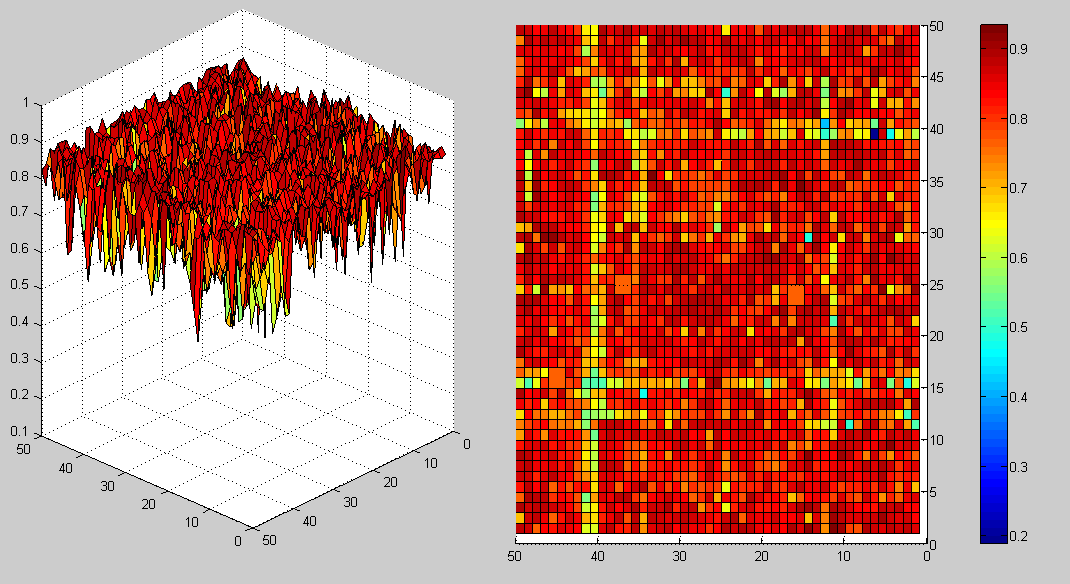
\includegraphics[height=90mm]{6-out-topology.png}}
  \caption{Isometric and top-down view of surface created by plotting neurons per layer \\ against average $F_1$ value for six-output tree}
\end{figure}

\begin{figure}[p]
  \centering
  {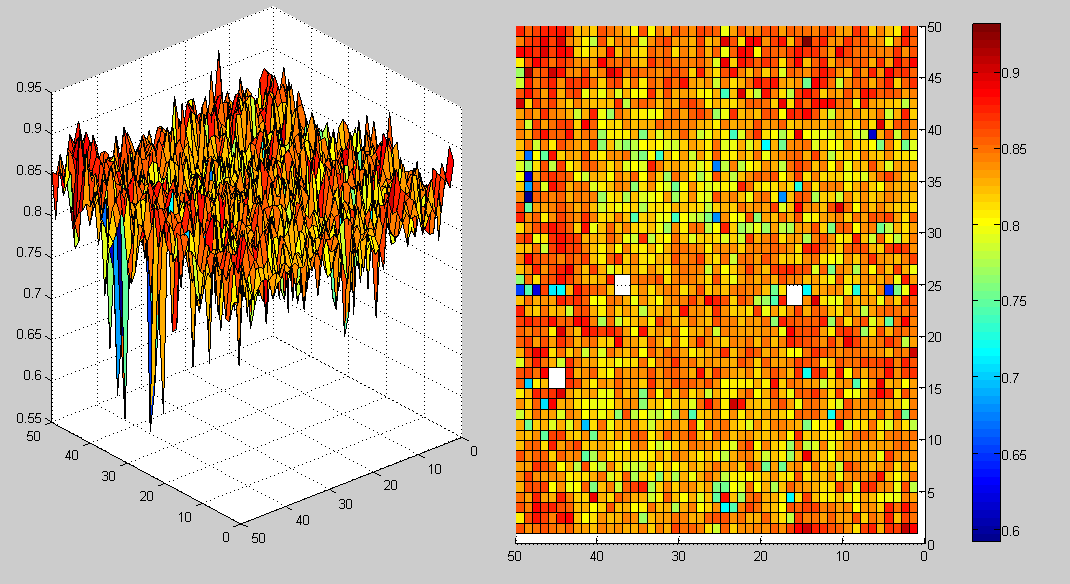
\includegraphics[height=90mm]{1-out-topology.png}}
  \caption{Isometric and top-down view of surface created by plotting neurons per layer \\ against average $F_1$ value for single-output trees}
\end{figure}

\begin{landscape}
\begin{figure}[p]
  \centering
  {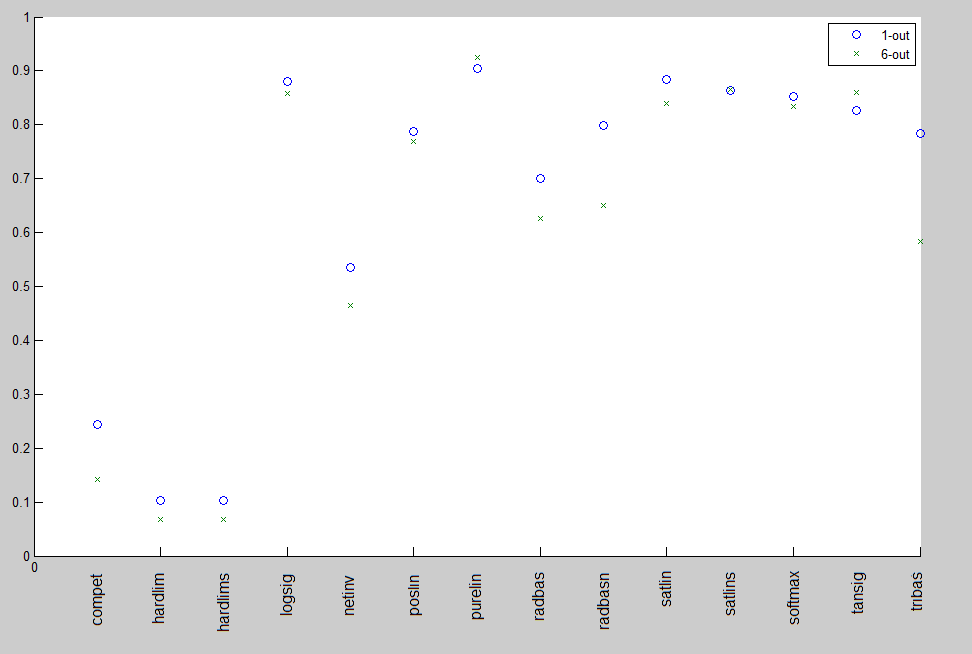
\includegraphics[height=120mm]{transfer-function.png}}
  \caption{Results of varying transfer function used}
\end{figure}

\begin{figure}[p]
  \centering
  {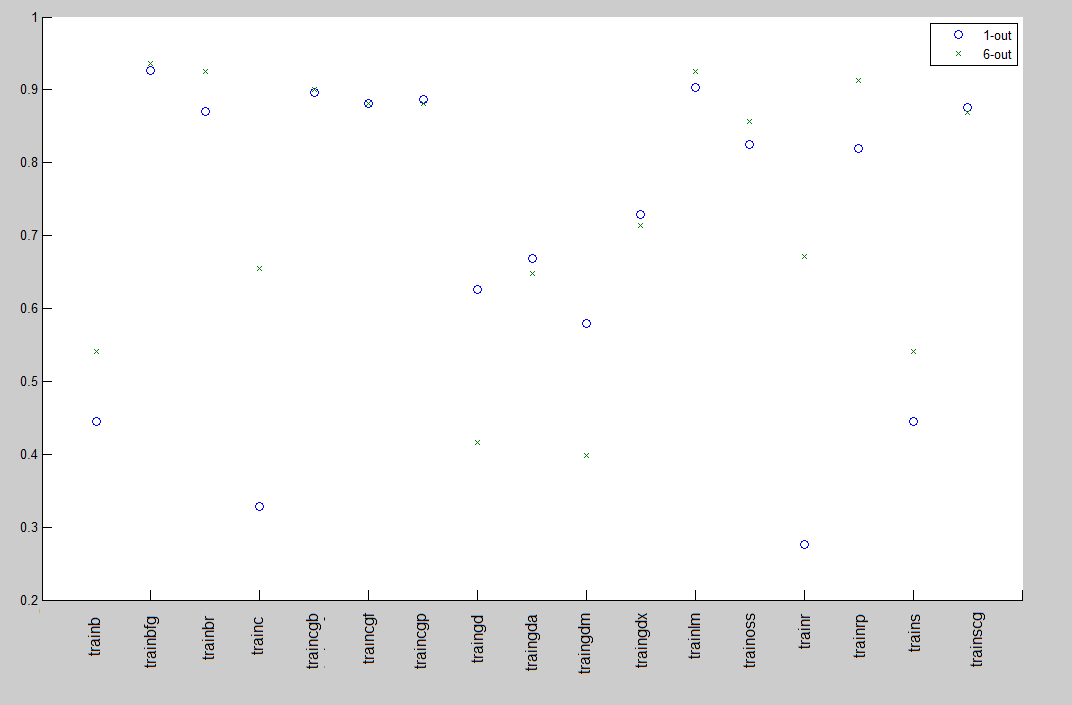
\includegraphics[height=120mm]{training-function.png}}
  \caption{Results of varying training function used (constant learning rate)}
\end{figure}
\end{landscape}

\end{document}